\documentclass[a4paper,oneside,14pt]{extreport}

\usepackage[T2A]{fontenc}
\usepackage[utf8]{inputenc}
\usepackage[english,russian]{babel}

%\usepackage[left=30mm, right=20mm, top=20mm, bottom=20mm]{geometry}
\usepackage[left=20mm, right=10mm, top=5mm, bottom=20mm]{geometry}

\usepackage{microtype}
\sloppy

\usepackage{setspace}
\onehalfspacing

\usepackage{indentfirst}
\setlength{\parindent}{12.5mm}

\usepackage{titlesec}
\titleformat{\chapter}{\LARGE\bfseries}{\thechapter}{14pt}{\LARGE\bfseries}
\titlespacing*{\chapter}{\parindent}{0mm}{5mm}
\titleformat{\section}{\Large\bfseries}{\thesection}{14pt}{\Large\bfseries}

\addto{\captionsrussian}{\renewcommand*{\contentsname}{Содержание}}
\usepackage{natbib}
\renewcommand{\bibsection}{\chapter*{Список использованных источников}}

\usepackage{caption}

\usepackage{wrapfig}
\usepackage{float}

\usepackage{graphicx}
\newcommand{\imgwc}[4]
{
	\begin{figure}[#1]
		\center{\includegraphics[width=#2]{inc/img/#3}}
		\caption{#4}
		\label{img:#3}
	\end{figure}
}
\newcommand{\imghc}[4]
{
	\begin{figure}[#1]
		\center{\includegraphics[height=#2]{inc/img/#3}}
		\caption{#4}
		\label{img:#3}
	\end{figure}
}
\newcommand{\imgsc}[4]
{
	\begin{figure}[#1]
		\center{\includegraphics[scale=#2]{inc/img/#3}}
		\caption{#4}
		\label{img:#3}
	\end{figure}
}

\usepackage{pgfplots}
\pgfplotsset{compat=newest}

\usepackage{listings}
\usepackage{listingsutf8}
\lstset{
	basicstyle=\footnotesize\ttfamily,
	keywordstyle=\color{blue},
	stringstyle=\color{red},
	commentstyle=\color{gray},
	numbers=left,
	numberstyle=\tiny,
	numbersep=5pt,
	frame=false,
	breaklines=true,
	breakatwhitespace=true,
	inputencoding=utf8/koi8-r
}

\lstdefinestyle{c}{
	language=C++,
	backgroundcolor=\color{white},
	basicstyle=\footnotesize\ttfamily,
	keywordstyle=\color{blue},
	stringstyle=\color{red},
	commentstyle=\color{gray},
	directivestyle=\color{orange},
	numbers=left,
	numberstyle=\tiny,
	stepnumber=1,
	numbersep=5pt,
	frame=single,
	tabsize=4,
	captionpos=t,
	breaklines=true,
	breakatwhitespace=true,
	escapeinside={\#*}{*)},
	morecomment=[l][\color{magenta}]{\#},
	columns=fullflexible
}

\newcommand{\code}[1]{\texttt{#1}}

\usepackage{amsmath}
\usepackage{amssymb}

\usepackage[unicode]{hyperref}
\hypersetup{hidelinks}

\makeatletter
\newcommand{\vhrulefill}[1]
{
	\leavevmode\leaders\hrule\@height#1\hfill \kern\z@
}
\makeatother

\begin{document}

\begin{titlepage}
	\centering
	
	\vspace{-2.2mm}
	\vhrulefill{0.9mm}\\
	\vspace{-7mm}
	\vhrulefill{0.2mm}\\
	\vspace{2mm}
	
	\vspace{50mm}
	
	\vspace{30mm}
	
	\textbf{Отчет по лабораторной работе №7}\\
	По курсу: <<Фильтрация и прогнозирование данных>>\\
	Тема: <<Решение обратной задачи>>\\
	
	\vspace{60mm}
	
	\hspace{70mm} Студент:       \hfill Пронин~А.~С.\\
	\hspace{70mm} Группа:        \hfill МСМТ231\\
	\hspace{70mm} Преподаватель: \hfill Зотов~Л.~В.\\
	%	\hspace{70mm} Оценка:        \hfill \hrulefill\\
	
	\vfill
	
	Москва\\
	\the\year
\end{titlepage}

\setcounter{page}{2}

\chapter*{Лабораторная работа 3}

Задание 1 – Добавить к сигналу из ЛР N1 авторегрессионный шум

Исходный сигнал из ЛР 1 (рис. \ref{lr1_signal}):

\begin{figure}[!h]
	\center{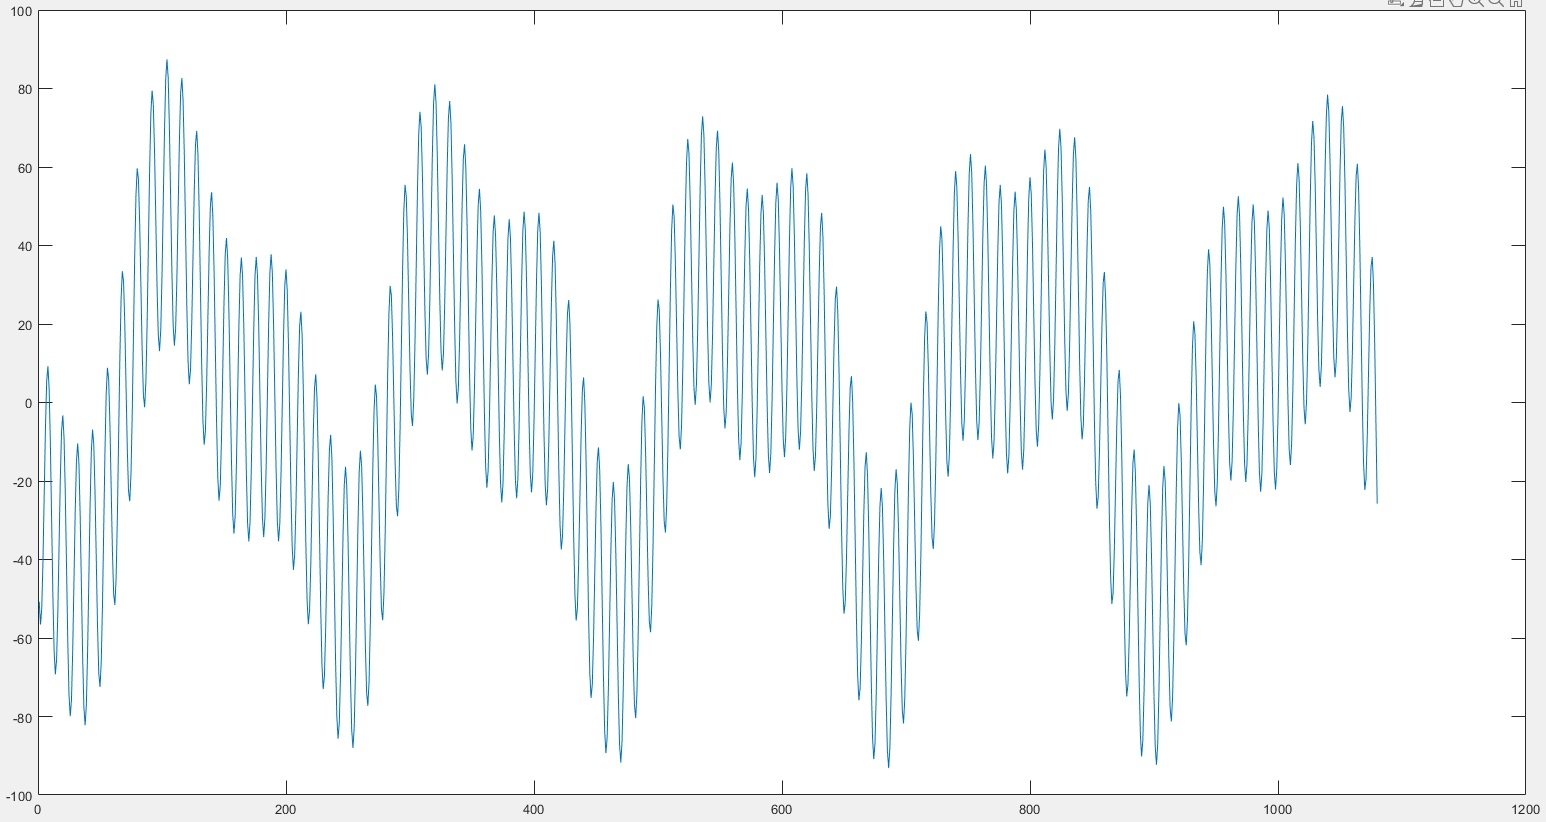
\includegraphics[width=1\linewidth]{inc/lr1_signal}}
	\caption{Исходный сигнал из ЛР 1}
	\label{lr1_signal}
\end{figure}

\newpage
Добавим к нему авторегрессионный шум (рис. \ref{task1_shum1}-\ref{task1_signal_shum1}):

\begin{figure}[!h]
	\center{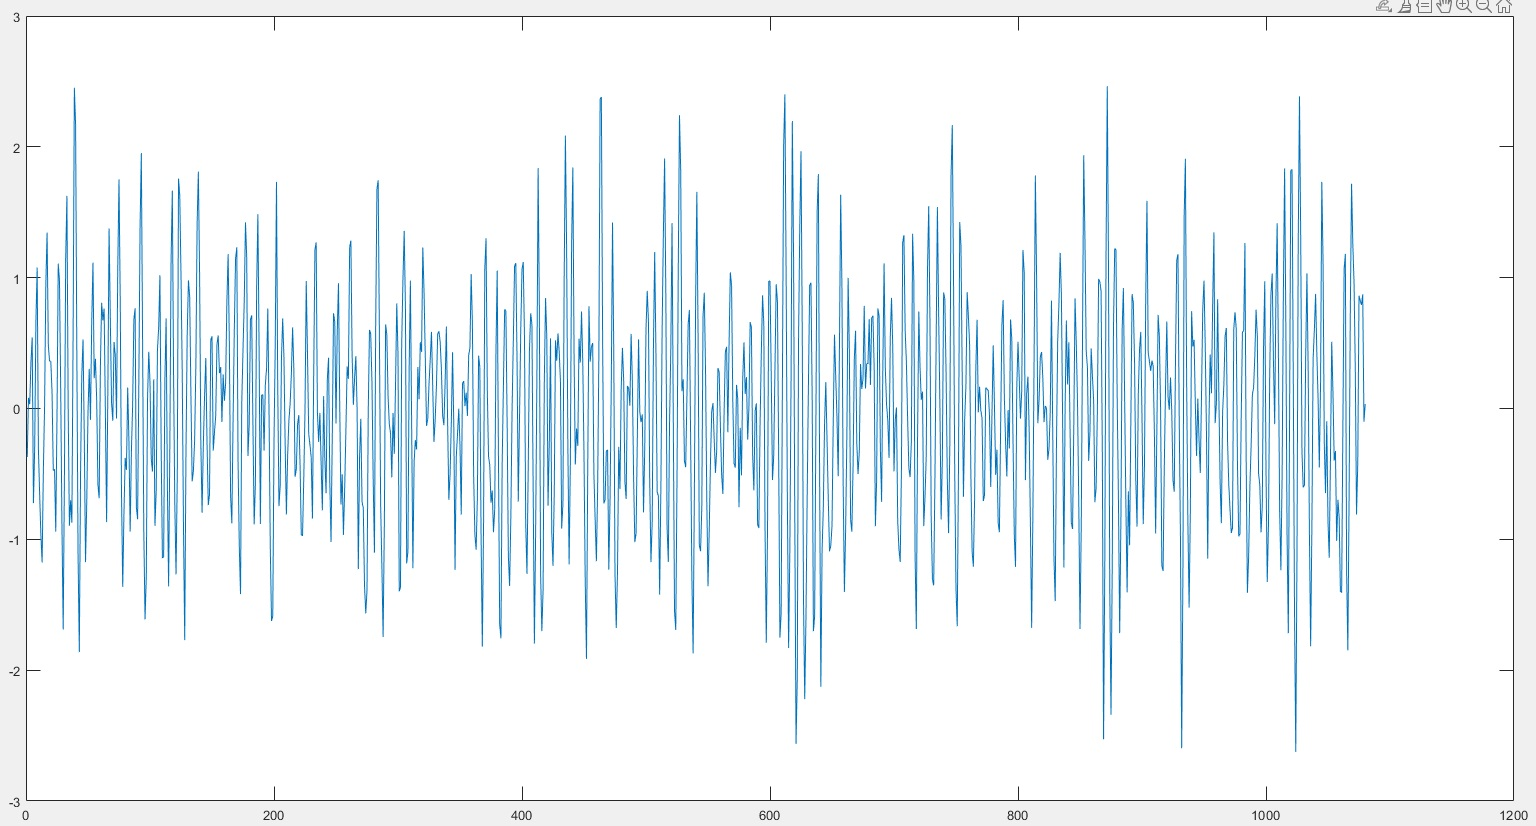
\includegraphics[width=1\linewidth]{inc/task1_shum1}}
	\caption{Шум 1}
	\label{task1_shum1}
\end{figure}

\begin{figure}[!h]
	\center{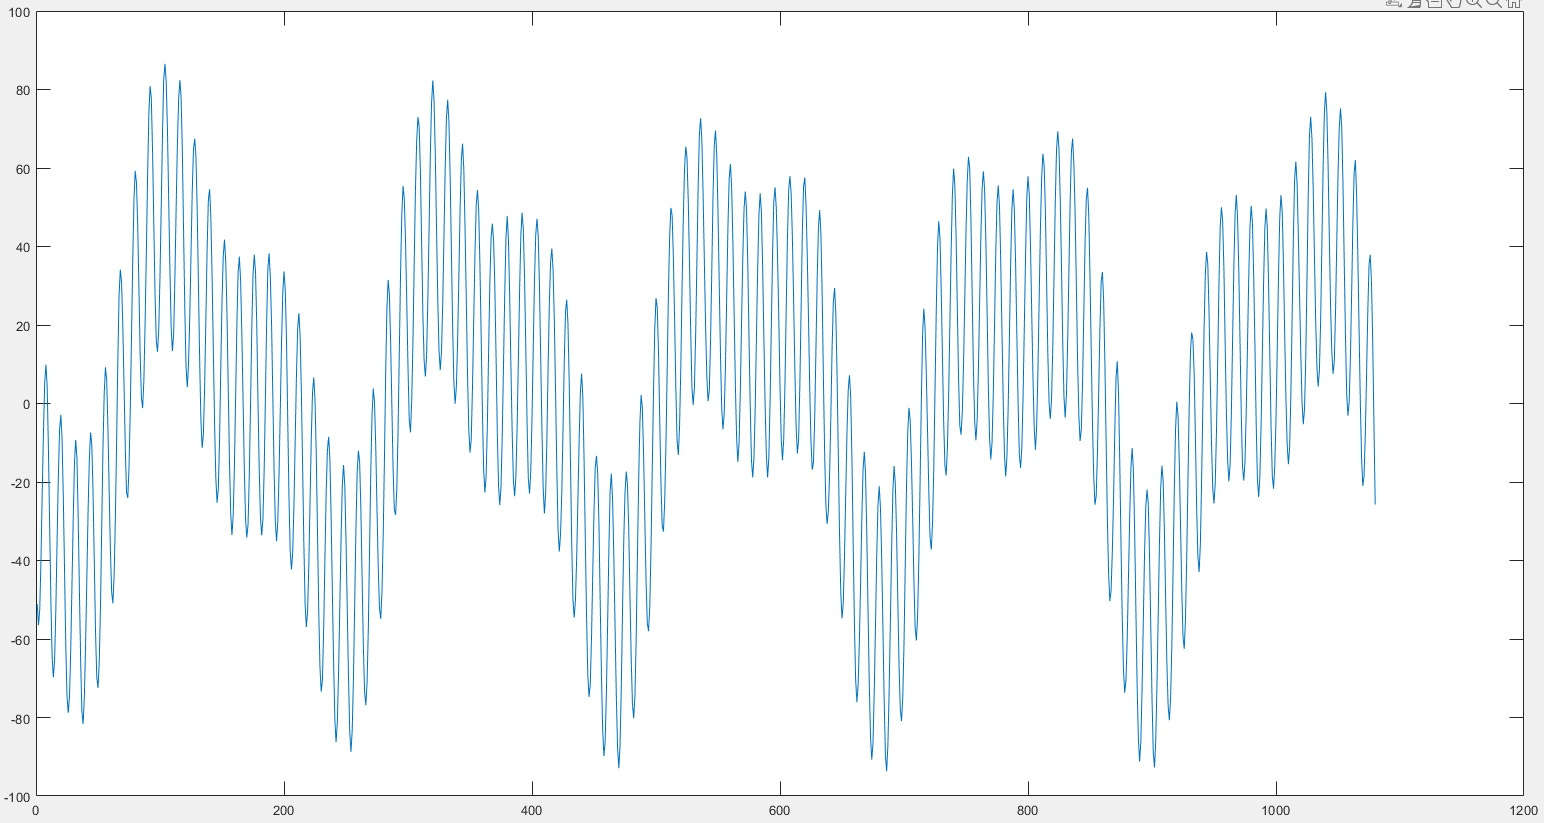
\includegraphics[width=1\linewidth]{inc/task1_signal_shum1}}
	\caption{Сигнал с шумом 1}
	\label{task1_signal_shum1}
\end{figure}

\newpage
По графикам \ref{task1_shum1}-\ref{task1_signal_shum1} видно, что сигнал почти не изменился, поэтому увеличим разброс шума (рис. \ref{task1_shum2}-\ref{task1_signal_shum2}):

\begin{figure}[!h]
	\center{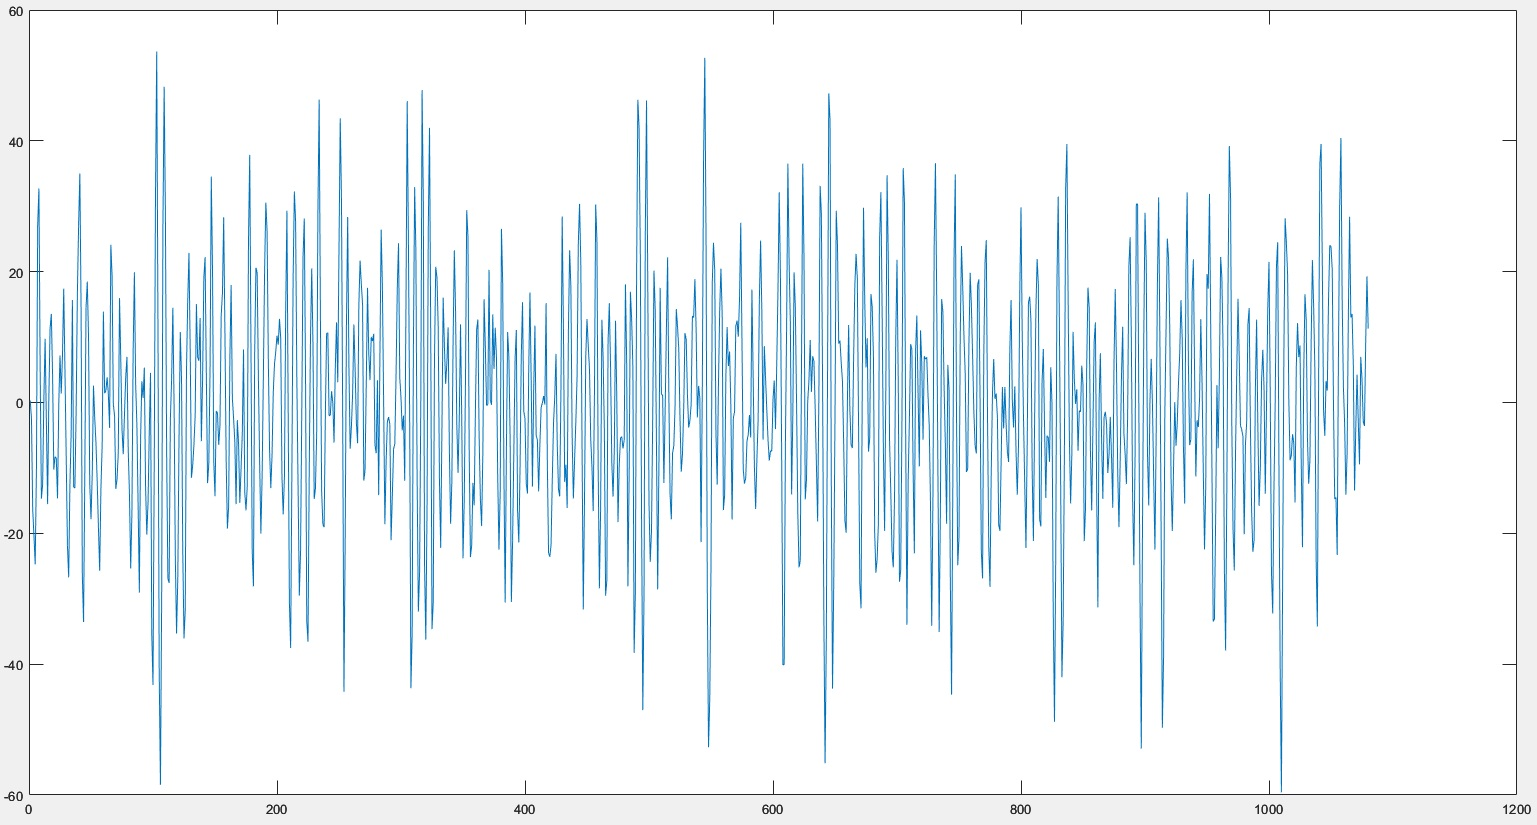
\includegraphics[width=1\linewidth]{inc/task1_shum2}}
	\caption{Шум 2}
	\label{task1_shum2}
\end{figure}

\begin{figure}[!h]
	\center{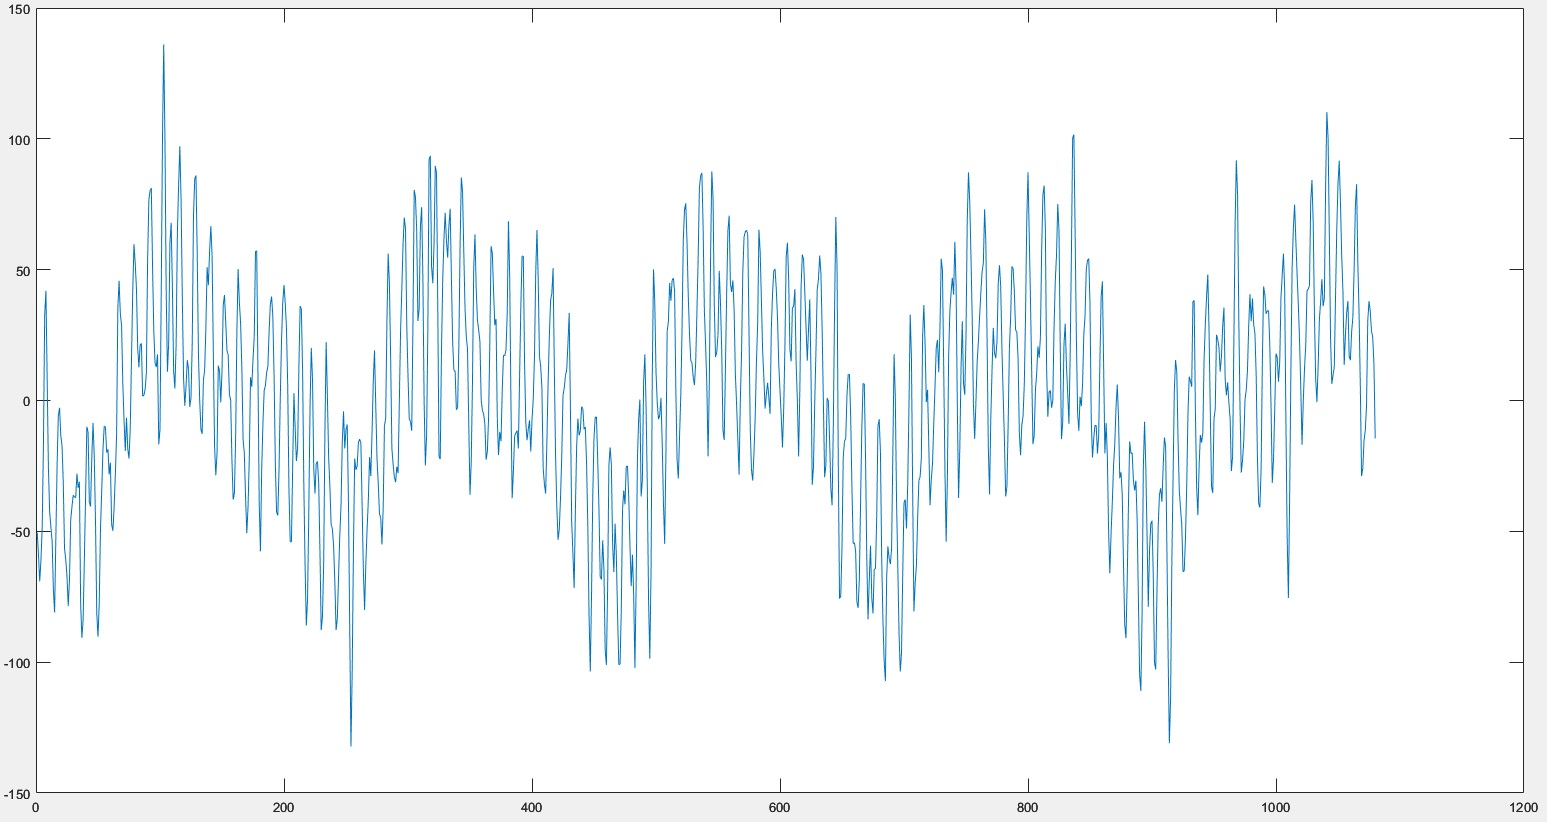
\includegraphics[width=1\linewidth]{inc/task1_signal_shum2}}
	\caption{Сигнал с шумом 2}
	\label{task1_signal_shum2}
\end{figure}

\newpage
По заданию 2 сохраним полученный сигнал в файл signal.mat и обработаем его с помощью Wavelet Analyzer (рис. \ref{task5}):

\begin{figure}[!h]
	\center{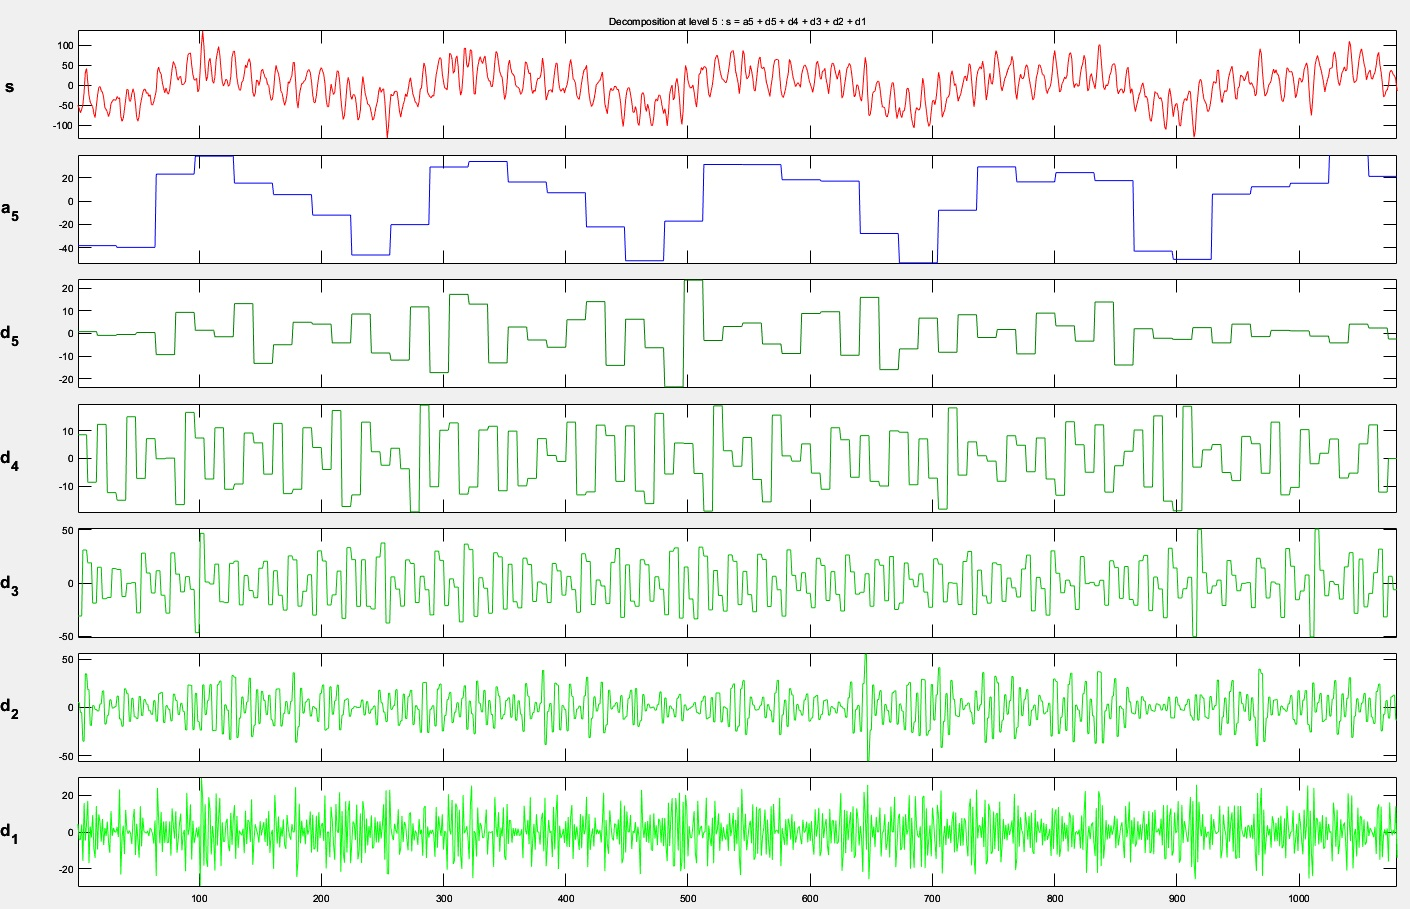
\includegraphics[width=1\linewidth]{inc/task5}}
	\caption{Wavelet Analyzer}
	\label{task5}
\end{figure}

Используем старую версию cwt для нашего сигнала (рис. \ref{task2}):

\begin{figure}[!h]
	\center{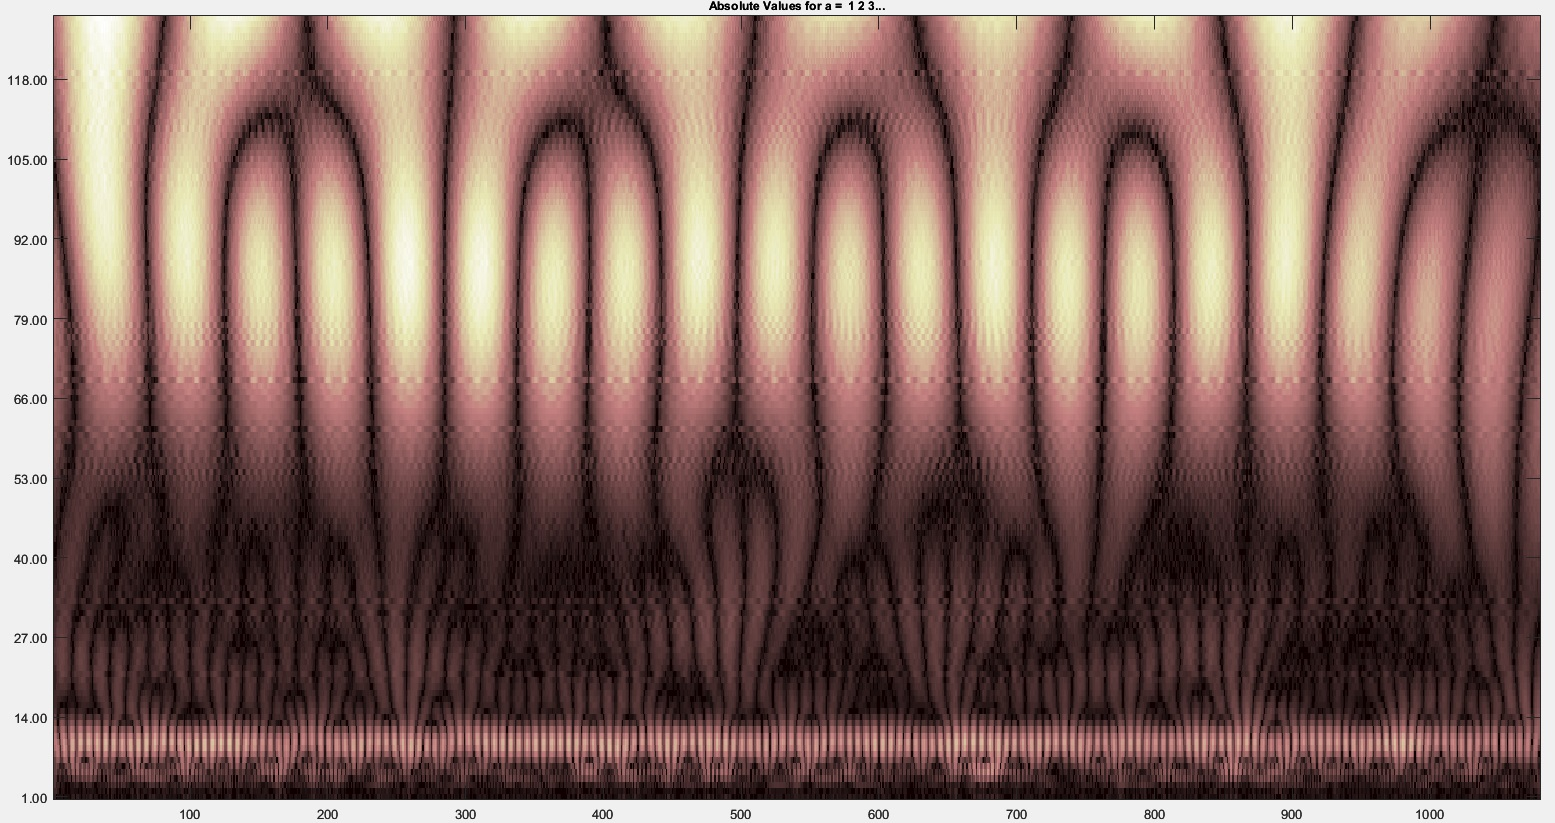
\includegraphics[width=1\linewidth]{inc/task2}}
	\caption{Старая версия cwt}
	\label{task2}
\end{figure}

\newpage
На рисунке \ref{task2} можно увидеть что в результате Вейвлет анализа отобразилась информация как о низких, так и о высоких частотах. Изучив коэффициенты вейвлет-преобразования, можно выделить частотные компоненты сигнала. Это позволяет локализовать и анализировать различные частоты в сигнале.

По заданию 4 построим 3D поверхность для данной скалограммы (рис. \ref{task4}):

\begin{figure}[!h]
	\center{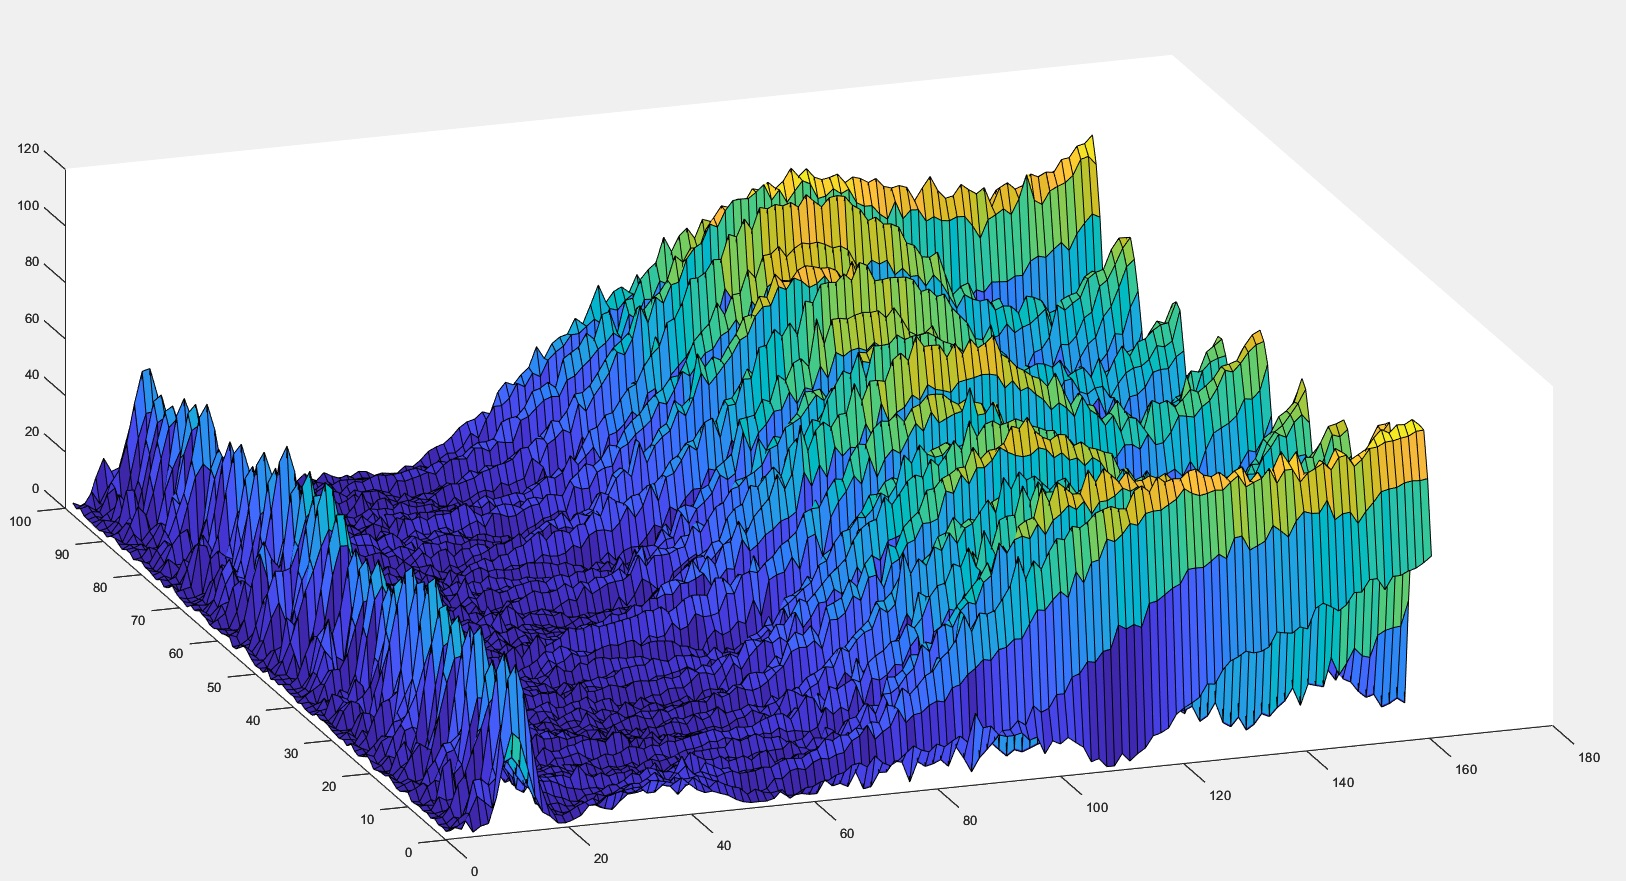
\includegraphics[width=1\linewidth]{inc/task4}}
	\caption{3D поверхность}
	\label{task4}
\end{figure}

\newpage
По заданию 6 добавим импульс в сигнал для сотого элемента и изучим треугольник его влияния (рис. \ref{task6}):

\begin{figure}[!h]
	\center{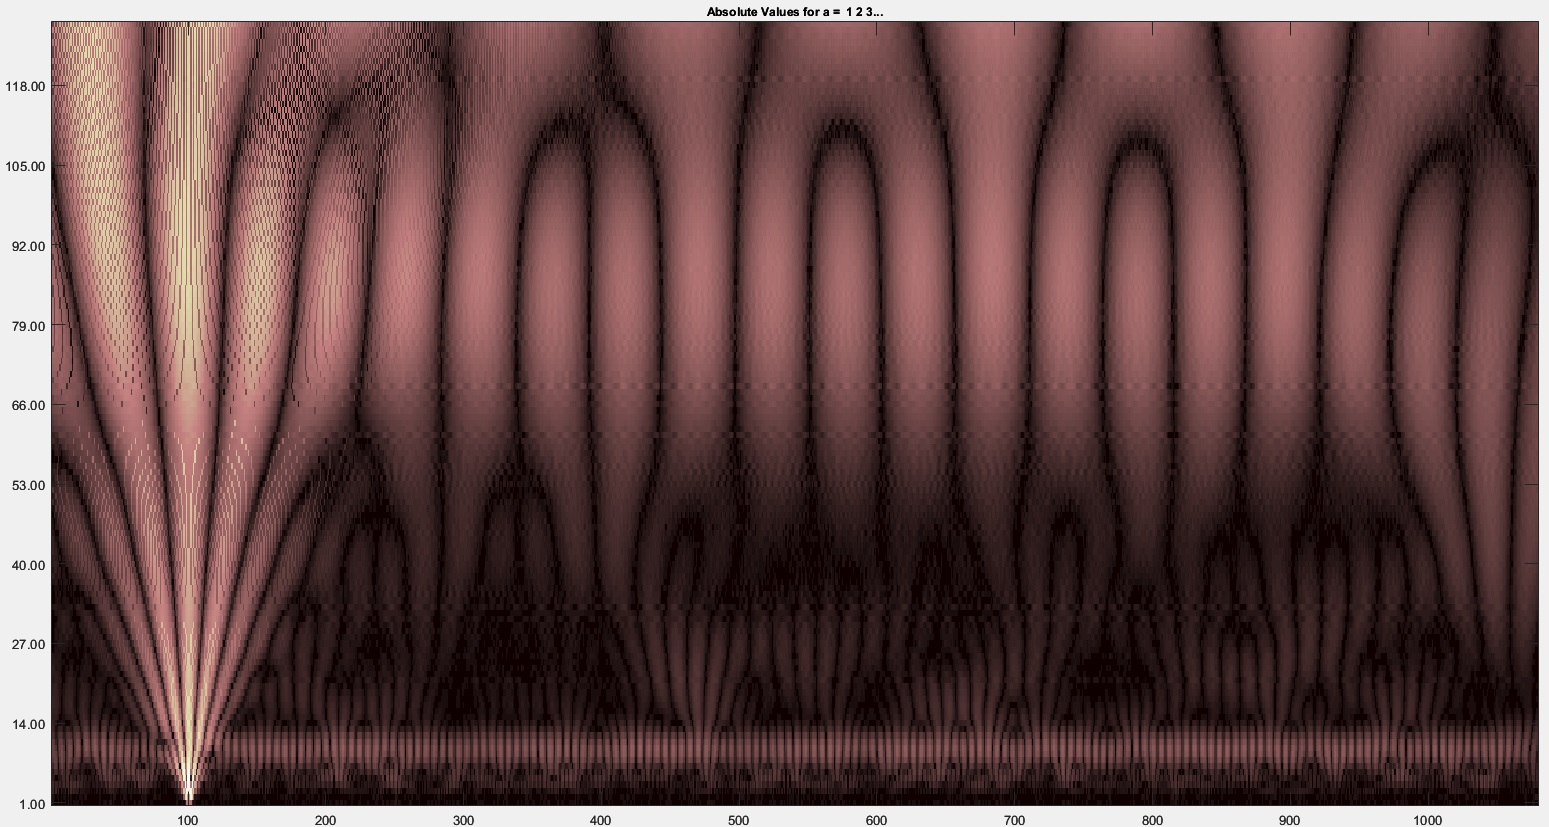
\includegraphics[width=1\linewidth]{inc/task6}}
	\caption{Вейвлет анализ сигнала с импульсом}
	\label{task6}
\end{figure}

Как видно по рисунку \ref{task6}, как и ожидалось, треугольник исходящий из сотого элемента выделяется среди других. Из этого можно сделать вывод что Вейвлет анализ также предоставляет информацию о локальных изменениях в сигнале, что помогает выявлять переходы между различными участками сигнала и определять их структуру.

\newpage
По заданию 7 выполним Вейвлет анализ сигнала LOD из файла eopc\_C02.dat (рис. \ref{task7}):

\begin{figure}[!h]
	\center{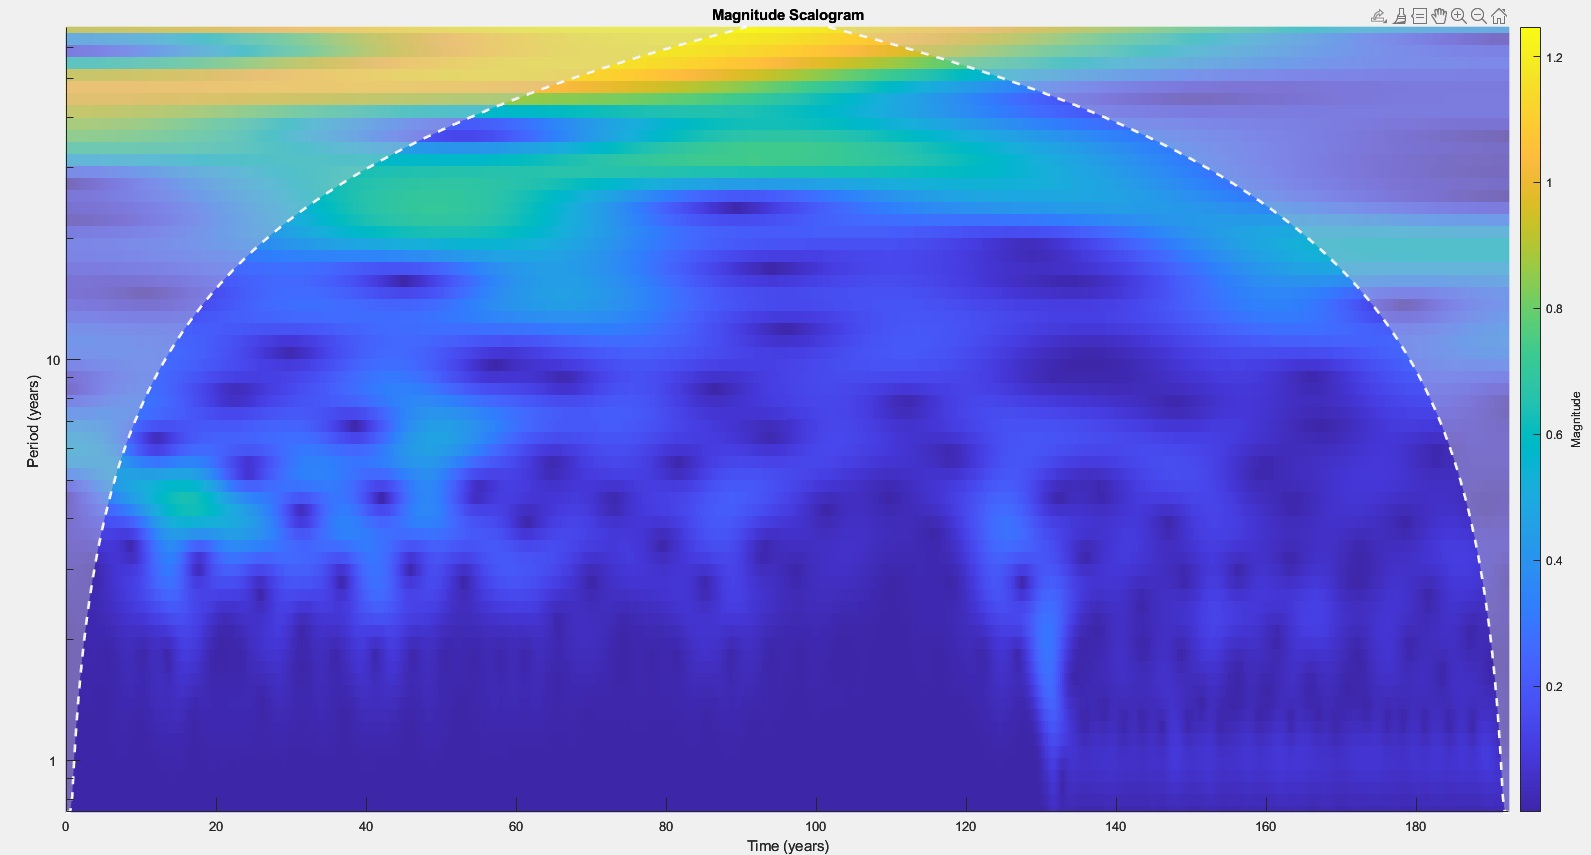
\includegraphics[width=1\linewidth]{inc/task7}}
	\caption{Вейвлет анализ сигнала LOD из файла eopc\_C02.dat}
	\label{task7}
\end{figure}

\end{document}